%
% TODO Sashank's and Nakayama's environmental, repair transitions and numerical
% optimizations (U/D states). Talk about environment dependent phis in Remarks?
% phi pinching

\documentclass[12pt]{article}

\usepackage{graphicx,amsmath}
\usepackage{algorithm}
\usepackage{algorithmic}
\usepackage{mathabx}
\usepackage[left = 1.0in, top = 1in, right = 1.0in, bottom = 1in, nohead]{geometry}
\usepackage{color}
\usepackage{ulem}
\usepackage{tikz}
\usepackage{pgfplots}
\usepackage{caption}
\usetikzlibrary{arrows}

\def\myxout{\bgroup \markoverwith{\textcolor{red}{\hbox to.35em{\hss/\hss}}}\ULon}
\def\myxoutii{\bgroup \markoverwith{\textcolor{blue}{\hbox to.35em{\hss/\hss}}}\ULon}

\usepackage{ifthen}

\newboolean{booleanfinal}

% Comment out one of the following lines. If booleanfinal = true, then changes are % not highlighted.
% \setboolean{booleanfinal}{true}
\setboolean{booleanfinal}{false}

\ifthenelse{\boolean{booleanfinal}}
{
  \newcommand{\deleted}[1]{}
  \newcommand{\changed}[1]{#1}
  \newcommand{\deletedii}[1]{}
  \newcommand{\changedii}[1]{#1}
}
{
  \newcommand{\changed}[1]{\textcolor{red}{#1}}
  \newcommand{\deleted}[1]{{\myxout{#1}}}

  \newcommand{\changedii}[1]{\textcolor{blue}{#1}}
  \newcommand{\deletedii}[1]{{\myxoutii{#1}}}

}

\newcommand{\captionAmerica}[2]{\noindent\hrLine\vspace{-0.25em}\\*{\raggedright\textbf{Algorithm #1} #2}\vspace{-0.8em}\\*\hrLine}
\newcommand{\hrLine}{\hspace{\fill}\rule{1.0\linewidth}{0.7pt}\hspace{\fill}}
\newcommand{\varName}[1]{\textrm{\it#1}}
\newcommand{\citeLine}[1]{$\langle \, #1 \, \rangle$}
\newcommand{\citeBlock}[2]{$\langle \, #1 - #2 \, \rangle$}
\newcommand{\nodeLabel}[2]{\mbox{$#1$-$#2$}}
\newcommand{\modelgraphlabel}[4]{$#1$ \\ $r=#2$ \\ $q=#3$ \\ $\lambda=#4$}
\newcommand{\scale}{8}

\begin{document}
\title{Efficient Algorithms for
Analyzing Cascading Failures in a
Markovian Dependability Model}
\author{Mihir Sanghavi, Sashank Tadepalli, 
and Marvin K. Nakayama
\\
Computer Science Department
\\
New Jersey Institute of Technology
\\
Newark, NJ \ 07102}
\date{}
\maketitle

\abstract{
We develop an efficient algorithm to
construct and solve 
a Markovian dependability system
with cascading failures.
Our algorithm reduces runtimes by
orders of magnitude compared to a
previous method.
We also develop some heuristics
to further reduce the computational efforts
by instead constructing an approximate
model.  We present numerical results
demonstrating the effectiveness of our
approaches.
}


\section{Introduction}
\label{sec:intro}

Modern society relies on
complex stochastic systems that operate
in uncertain environments.
These systems can suffer from
cascading failures, in which
the failure of one part of the
system causes other parts to
also fail.
Examples include
networks
\cite{CLM:2004},
electric power grids
\cite{CLDN:2002},
national infrastructures
\cite{Little:2002},
and
transportation and communication systems
\cite{ZGZ:2007}.
Cascading failures in these
systems can be catastrophic,
causing widespread disruptions and
damage.


In this paper we develop methods for
analyzing a dependability
system with cascading failures.
We model such a system as 
a continuous-time
Markov chain (CTMC; e.g., Chapter~5 of
\cite{Ross:1995}),
where the system is 
a collection
of components operating
in a randomly changing environment, 
where each component can
fail and be repaired with
specified failure and repair rates.
% We allow for cascading failures, where the
% failure of one component can
% probabilistically 
% cause other
% components to simultaneously fail.
We represent a cascading failure as
a tree of probabilistically
failing components that fail
simultaneously, where the
root of the tree is the
failing component that 
\textit{triggers}
the cascade.  The root probabilistically
causes components from a specified
set to
fail simultaneously, with
each component in the set having
its own \textit{component-affected 
probability}.
Each of these secondary
failures subsequently
cause other components to
probabilistically fail simultaneously,
and so on.
The \textit{rate} of
the resulting tree depends on the
failure rate of the root and the
component-affected probabilities
of the failing and non-failing components
in the cascade.

Analyzing such a Markovian dependability
model with cascading failures
presents significant challenges.
Even simply
building the infinitesimal
generator matrix $Q$ of the
CTMC can be extremely time consuming,
and indeed, the amount of work required
can grow exponentially in the number
of components in the system.
For example, consider a simple
system with components $A$, $B$ and $C$,
where the failure of any one component
can cause each of the others
to fail simultaneously with certain
probabilities.
For a CTMC transition $(x,y)$ in which
all three components fail simultaneously,
there are $9$ corresponding
cascading-failure 
trees:
$A$ causing $B$ to fail, and then $B$
causes $C$ to fail;
$A$ causing $B$ and $C$ to simultaneously fail;
$B$ causing $A$ causing $C$ to fail;
and so on.
If the different
components' failure rates
and the component-affected probabilities
differ, then each of the $9$ trees
has a different rate,
and 
computing the $(x,y)$-entry in $Q$
requires summing the rates
of all $9$ trees.
In general, the number of trees
corresponding to a single collection
of components simultaneously failing
can grow exponentially in the size of the
set \cite{ING:2009}.  
Moreover, we need to examine
each possible set of components
that can simultaneously fail,
and the number of such
sets is exponential in the number
of components in the system.
Thus, just constructing the $Q$-matrix
for the CTMC can require tremendous
computational effort.

The paper \cite{ING:2009} 
considers the same dependability model
and develops
an algorithm to generate the $Q$-matrix,
but that algorithm
there often requires enormous
runtimes to build and solve larger models.  
We now develop
new algorithms, which are significantly
more efficient and can decrease the
computational effort by orders of magnitude.
We have developed software
implementing our techniques,
and we call the package
the Dependability Evaluator
of Cascading Failures (DECaF).

In addition, since the time to 
construct the $Q$-matrix 
inherently grows exponentially,
we also propose heuristics
to reduce the
computational effort by only 
generating a subset of the trees.
The omission
leads to an approximate $Q$-matrix,
which incurs errors in 
the resulting dependability measures.
We explore the trade-off
of the time savings from
skipping trees
with the error in the dependability
measures.

Previous tree-generation
algorithms exist (e.g.,
Section 2.3.4.4 of \cite{Knut:1997})
for enumerating
all possible trees in which there are
no limitations on a node's possible
children.
But in our model,
we restrict the
children a particular node
can have,
which is why \cite{ING:2009}
and the current paper
needed to develop
new tree-generation
algorithms.



The rest of the paper has the
following layout.
Section~\ref{sec:prior} reviews
related work on 
dependability models,
with a particular focus
on cascading failures
and other component interactions.
We describe the model
in Section~\ref{sec:model}.
% and the corresponding CTMC
% in Section~\ref{sec:ctmc}.
Section~\ref{sec:alg} describes
our new algorithms to build
the CTMC's $Q$-matrix and presents
numerical results comparing its
runtime to that of the implementation
in \cite{ING:2009}.
In Section~\ref{sec:approx}
we develop our various heuristics
that reduce runtime by not
generating all trees at the
expense of introducing error
in the dependability measures,
and we explore the trade-off
through experiments.
We apply our methods to 
a large cloud-computing model
in Section~\ref{sec:cloud},
and Section~\ref{sec:conc}
ends the paper with some
concluding remarks.



\section{Related Work}
\label{sec:prior}

As mentioned in Section~\ref{sec:intro},
the model we consider was previously
studied in \cite{ING:2009}, but
our new algorithms can solve large
models with orders-of-magnitude
reductions in runtime.
The SAVE (System Availability Estimator)
package \cite{BHLNS:1994}, developed at IBM,
analyzes a similar Markovian dependability
model with cascading failures
having the restriction that there
is only one level of cascading;
i.e., the root of a tree can
cause other components to simultaneously
fail, but those subsequent failures
cannot cause further failures.
Allowing for more than a
single level of cascading
makes the CTMC model we consider
tremendously more
difficult to construct.

Other modeling techniques,
such as fault trees, reliability
block diagrams (RBDs), and reliability graphs,
have also been applied to study 
dependability systems, but these
approaches do not allow for 
the level of details that are
possible with CTMCs \cite{MFT:2000}.  
However,
a notable drawback of CTMCs is the
explosive growth in the size of the
state space, which increases exponentially
in the number of components in the system.
Other packages for analyzing Markovian
dependability models include
SHARPE \cite{STP:1996},
SURF \cite{Butl:1986},
SURF-2 \cite{SURF2:1993},
TANGRAM \cite{BSM:1991},
and HIMAP \cite{KGS:1996}.

Instead of assuming a Markovian
system, some packages work with
other mathematical models, such as
stochastic Petri nets,
which are analyzed by SNPN
\cite{HTT:2000}.
OpenSESAME \cite{WSB:2008}
also solves stochastic Petri nets
described via a high-level
modeling language, which allows
for cascading failures through
failure dependency diagrams,
but the complexity of the
cascades that can be handled is
not as great as in our model.
The Galileo package
\cite{SDC:1999}
examines dynamic fault trees,
which can model certain types
of cascading failures via
functional dependency gates;
however, its modeling capability
is limited.
The paper \cite{LaPo:2007}
considers Bayesian networks
for studying reliability systems.

Other mathematical modeling techniques
that allow some forms of cascading
failures or component interactions
include Boolean driven
Markov processes (BDMP)
\cite{BoBo:2003},
common-cause and common-mode failures
\cite{ALRL:2004,BCS:1969},
and coverage
\cite{DuTr:1989}.
DRBD \cite{XXR:2009} uses
dynamic reliability block diagrams,
which extend traditional RBDs
to allow for certain component
interactions.

\section{Model}
\label{sec:model}

We work with the stochastic model of \cite{ING:2009}, which considers the
evolution over time of a repairable dependability system operating in a randomly
changing environment. The system consists of a collection $\Omega = \{ 1, 2,
\ldots, N \}$ of $N < \infty$ component types. Each component type $i \in
\Omega$ has a redundancy $1 \leq r_i < \infty$, and the $r_i$ components of
type~$i$ are assumed to be identical. A component can be either operational (up)
or failed (down).

The environment changes randomly within a set $\mathcal{E} = \{ 0, 1, 2, \ldots,
L \}$. For example, we can think of the environment as representing the current
load on the system, and if there are two possible environments, $0$ and $1$,
then $0$ (resp., $1$) may represent a low (resp., high) load. Once the
environment enters $e \in \mathcal{E}$, it remains there for an exponentially
distributed amount of time with rate $\nu_e > 0$, after which the environment
changes to $e'$ with probability $\delta_{e, e'} \geq 0$, where $\delta_{e, e} =
0$ and $\sum_{e' \in \mathcal{E}} \delta_{e, e'} = 1$. We assume the matrix
$\delta = (\delta_{e, e'} : e, e' \in \mathcal{E})$ is irreducible; i.e., for
each $e, e' \in \mathcal{E}$, there exists $k \geq 1$ and a sequence $e_0 = e,
e_1, e_2, \ldots, e_k = e'$ with each $e_i \in \mathcal{E}$ such that $\prod_{i
= 0}^{k-1} \delta_{e_i, e_{i + 1}} > 0$. In other words, it is possible to
eventually move from environment $e$ to environment $e'$.

The components in the system can randomly fail and then be repaired. When the
environment is $e \in \mathcal{E}$, the failure rate and repair rate of each
component of type $i$ are $\lambda_{i, e} > 0$ and $\mu_{i, e} > 0$,
respectively.  If there is only one environment $e$, i.e., $| \mathcal{E} | =
1$, then the lifetimes and repair times of components of type $i$ are
exponentially distributed with rates $\lambda_{i, e}$ and $\mu_{i, e}$,
respectively. Exponential distributions are frequently used to model lifetimes
of hardware and software components; e.g., see \cite{XDP:2004}. We assume that
all operating components of a type~$i$ have the same failure rate $\lambda_{i,
e}$ in environment $e$. Thus, in a system with  redundancies for which not all
components of a type are needed for operation of the system, the extras are
``hot spares'' since they fail at the same rate as the main components.

Our model includes probabilistic instantaneous cascading failures, which occur
as follows. The ordered set $\Gamma_i$ specifies the types of components that a
failure of a type-$i$ component can cause to simultaneously fail. When a
component of type $i$ fails, it causes a single  component of type~$j \in
\Gamma_i$ to fail at the same time with probability $\phi_{i, j}$ (if there are
components of type $j$ up), and we call 
$\phi_{i, j}$  a \textit{component-affected probability}. The events that the individual components of types $j \in
\Gamma_i$ fail immediately are independent. Thus, when a component of type $i$
fails, there are independent ``coin flips'' to determine which components in
$\Gamma_i$ fail, where the coin flip for $j \in \Gamma_i$ comes up heads (one
component of type $j$ fails) with probability $\phi_{i, j}$ and tails (no
components of type $j$ fail) with probability $1 - \phi_{i, j}$.

We allow for a cascading failure to continue as long as there are still
components operational in the system.  For example, the failure of a component
of type $i$ may cause a component of type $j$ to fail (with probability
$\phi_{i, j}$), which in turn makes a component of type $k$ fail (with
probability $\phi_{j, k}$), and so on. As noted in \cite{ING:2009}, the SAVE
package \cite{BHLNS:1994} allows for only one level of cascading, but the
unlimited cascading in our model makes it significantly more difficult to
analyze.

We can think of a cascading failure as a tree of simultaneously failing
components. The root is the component, say of type $i$, whose failure
\textit{triggers} the cascade. The root's children, which are from $\Gamma_i$,
are those components whose immediate failures were directly caused by the root's
failure. At any non-root level of the tree,  these components' failures were
directly caused by the failure of their parents at the previous level. Although
all the failing components in a cascade fail at the same time, we need to
specify an order in which they fail for our problem to be well-defined, as we
explain later in Section~\ref{sec:exrate}. We assume the components in a tree
fail in breadth-first order.

There is a single repairman who fixes failed components using a processor-
sharing discipline. Specifically, if the current environment is $e$ and there is
only one failed component, which is of type $i$, then the repairman fixes that
component at rate $\mu_{i, e}$. If there are $b$ components currently failed,
then the repairman allocates $1 / b$ of his effort to each failed component, so
a failed component of type $i$ is repaired at rate $\mu_{i, e}/b$.

\subsection{Markov Chain}
\label{sec:ctmc}

We want to analyze the behavior of the system as it evolves over time.  Because
of the processor-sharing repair discipline and the exponential rates for the
event lifetimes, it will suffice to define the state of the system as a vector
containing the number of failed components of each type and the current
environment. Thus, let $S = \{ x = (x_1, x_2, \ldots, x_N, x_{N + 1}) : 0 \leq
x_i \leq r_i \ \forall i \in \Omega, \, x_{N + 1} \in \mathcal{E} \}$ be the
state space, and let $Z = [Z(t) : t \geq 0]$ be the continuous-time Markov time
(CTMC) living on $S$ keeping track of the current state of the system. (If we
had instead considered a first-come-first-served repair discipline, then the
state space would need to be augmented to keep track of the order in which
current set of down components failed.) We assume that $Z$ starts in environment
$0 \in \mathcal{E}$ with no components failed, i.e., state $(0,0, \ldots, 0)$.
As noted in \cite{ING:2009} the CTMC is irreducible and positive recurrent.

We now describe the CTMC's infinitesimal generator matrix $Q = (Q(x, y) : x, y
\in S)$, where $Q(x, y)$ is the rate that the CTMC $Z$ moves from state $x =
(x_1, \ldots, x_N, x_{N + 1})$ to state $y = (y_1, \ldots, y_N, y_{N + 1})$. If
$y_i = x_i$ for each $i \in \Omega$ and $y_{N + 1} \neq x_{N + 1}$, then $(x,
y)$ is an \textit{environment transition} with $Q(x, y) = \nu_{x_{N + 1}}
\delta_{x_{N + 1},y_{N + 1}}$. If $y_i = x_i - 1$ for one $i \in \Omega$, $y_j =
x_j$ for each $j \in \Omega - \{ i \}$, and $y_{N + 1} = x_{N + 1}$, then $(x,
y)$ is a \textit{repair transition} corresponding to the repair of a component
of type $i$, and $Q(x, y) = x_i \mu_{i,x_{N + 1}}/(\sum_{j \in \Omega} x_j)$. If
$y_i \geq x_i$ for all $i \in \Omega$ with $y_j > x_j$ for some $j \in \Omega$
and $y_{N + 1} = x_{N + 1}$, then $(x, y)$ is a \textit{failure transition} in
which $y_i - x_i$ components of type~$i$ fail, $i \in \Omega$. Any other $(x,
y)$ with $x \neq y$ not falling into one of the above three categories is not
possible, so $Q(x, y) = 0$. The diagonal entry $Q(x, x) = -\sum_{y \neq x} Q(x,
y)$, as required for a CTMC; e.g., see Chapter~5 of 
\cite{Ross:1995}.

We now determine the rate $Q(x, y)$ of a failure transition $(x, y)$. First
consider the case when cascading failures are not possible, i.e., $\Gamma_i =
\emptyset$ for each type~$i$. Then the only possible failure transitions $(x ,
y)$ have $y_i = x_i + 1$ for one $i \in \Omega$, $y_j = x_j$ for each $j \in
\Omega - \{ i \}$, and $y_{N + 1} = x_{N + 1}$, and this corresponds to a single
component of type~$i$ failing. Then $Q(x, y) = (r_i - x_i) \lambda_{i, x_{N +
1}}$.

Cascading failures complicate the computation of $Q(x, y)$ for a failure
transition $(x, y)$. As mentioned before, a cascading failure is modeled as a
tree $T$ built from the multiset $B$ of simultaneously failing components, where
$B$ has $y_\ell - x_\ell$ failing components of type $\ell$, $\ell \in \Omega$.
A tree $T$ has a rate

\begin{equation}
\label{eq:rate}
R(T) = (r_i - x_i) \lambda_{i,x_{N + 1}} \, \rho \, \eta,
\end{equation}
where
\begin{itemize}
\item $(r_i - x_i) \lambda_{i,x_{N + 1}}$ is the failure rate of the root
(assumed here to be of type $i$),
\item $\rho = \rho(T)$ is the product of the
$\phi_{j, k}$ terms for a parent node of type $j$ causing a child of type $k \in
\Gamma_j$ to fail, and
\item $\eta = \eta(T,x)$ is the product of the $1 - \phi_{j, k}$ terms from a
node of type $j$ \textit{not} causing a component of type $k \in \Gamma_j$ to
fail when there are components of type $k$ up.
\end{itemize}

A difficulty arises since there can be many such trees corresponding to the
multiset $B$ of components failing in $(x, y)$, and calculating $Q(x, y)$
requires summing $R(T)$ over all possible trees $T$ that can be constructed from
$B$. The number of such trees grows exponentially in the number of failing
components in the cascade; see \cite{ING:2009}.

\subsection{Example of Computing a Tree's Rate}
\label{sec:exrate}

We now provide an example of computing the rate $R(T)$ of a tree $T$. Let
$\Omega = \{ A, B, C \}$, with $r_A = r_B = r_C = 4$. Also, let $\Gamma_A = \{
B, C \}$, $\Gamma_B = \{ A, C \}$, and $\Gamma_C = \{ A, B \}$. Suppose that
$\mathcal{E} = \{ 0 \}$, and consider the failure transition $(x, y)$ with $x =
(2, 2, 3, 0)$ and $y = (4, 4, 4, 0)$. Thus, $(x, y)$ corresponds to $2$
components each of types $A$ and $B$ failing and a single component of type $C$
failing. One possible tree $T$ corresponding to $(x, y)$ is shown in
Figure~\ref{fig:tree}. We assume the nodes in $T$ fail in breadth-first order.

\begin{figure}
\begin{center}
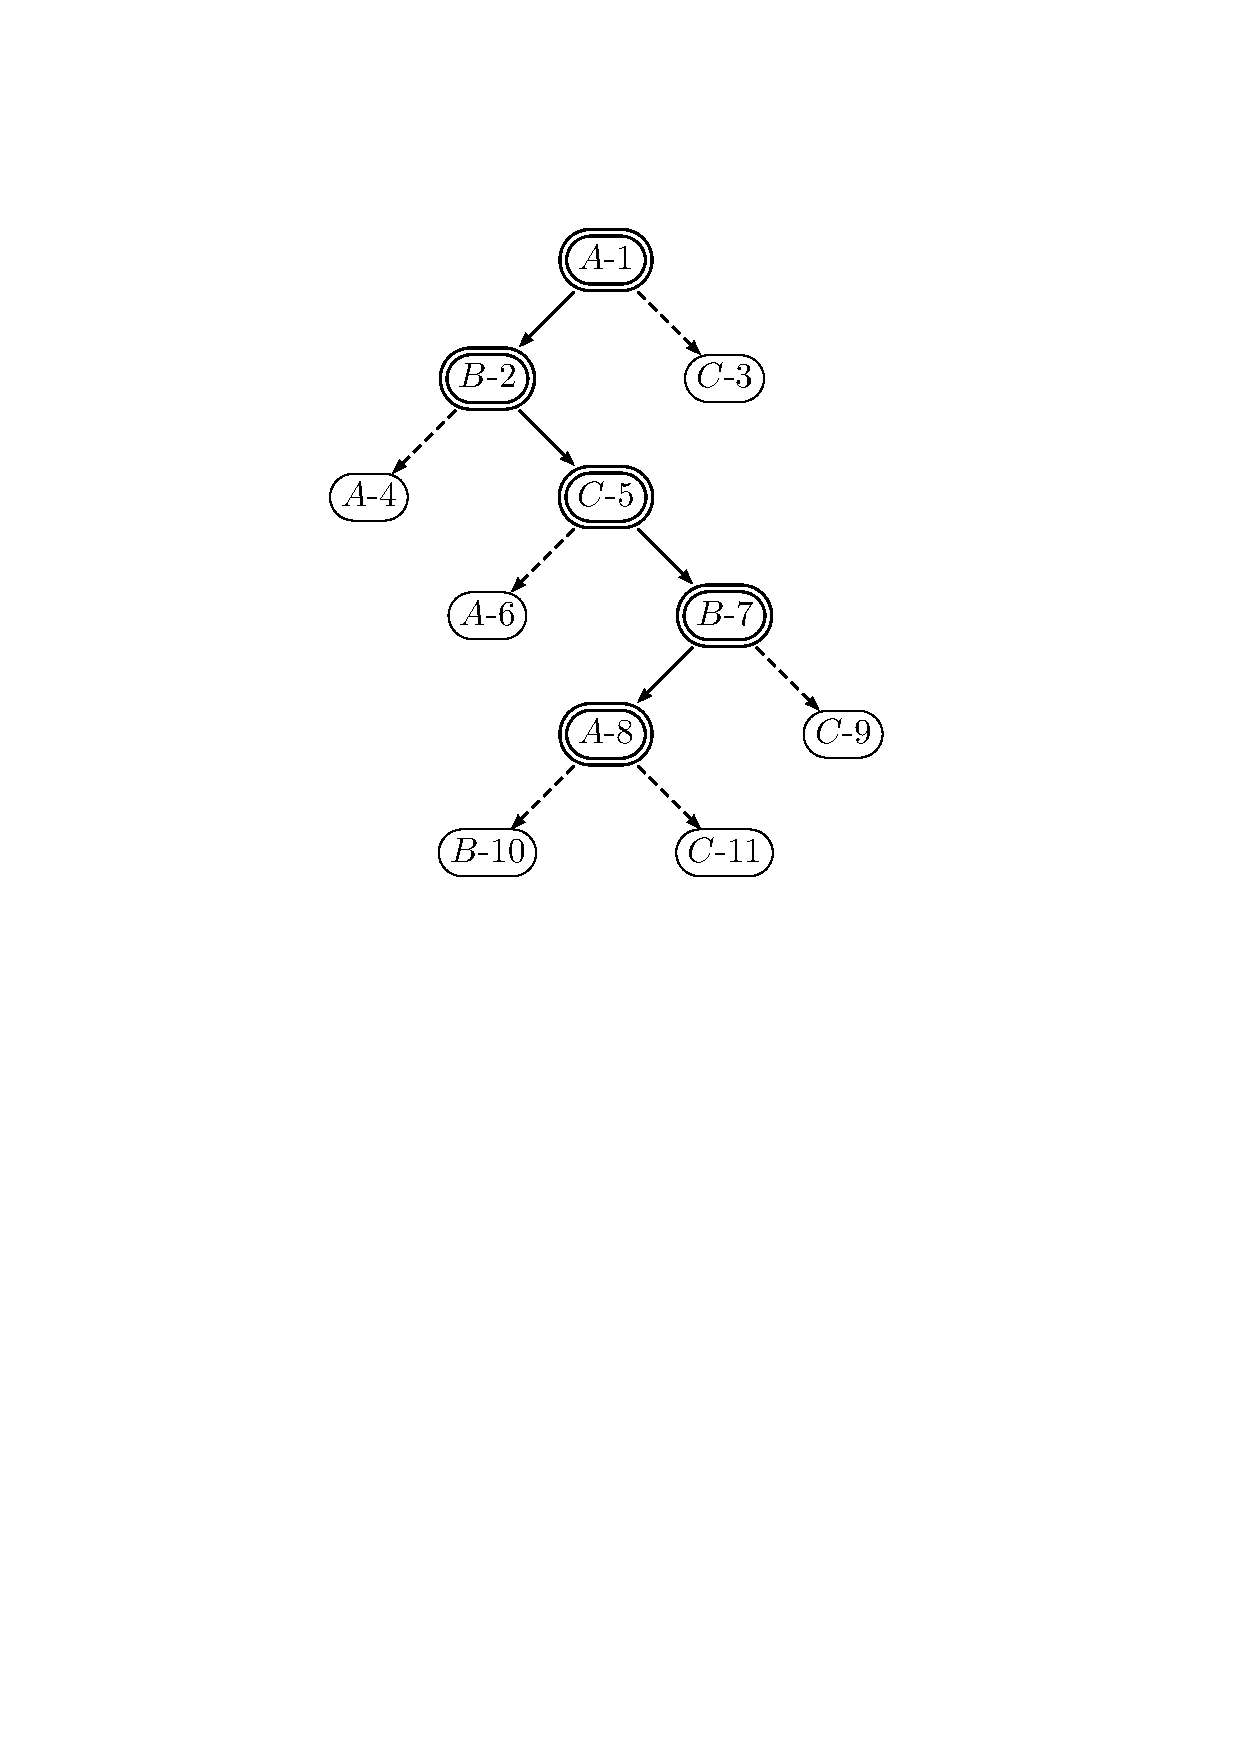
\includegraphics[width=0.4\textwidth]{fig_tree}
\end{center}
\caption{An example of a supertree.}
\label{fig:tree}
\end{figure}

The nodes depicted as double circles form the tree of failing components. The
single circles correspond to components in some $\Gamma_i$ but did not fail.  A
component type $j$ in some $\Gamma_i$ could have \textit{not failed} because
either there are components of type $j$ up at this point but its coin flip came
up tails (with probability $1 - \phi_{i, j}$), or there were no more components
of type $j$ up at this point. Each node has a label of the form $i$-ID, where
$i$ denotes the type of the component for that node, and ID is the position of
the node in a breadth-first ordering of all the nodes (single and double
circles). We include the IDs just to simplify the discussion here. We call the
tree of all nodes the \textit{supertree} corresponding to the tree $T$ of
failing nodes. The supertree is used to compute $R(T)$ of $T$ as follows. Let
$u_i$ be the number of components of type $i$ available in the system. Since the
root is a component of type $A$ and there are $u_A = r_A - x_A = 2$ components
of type $A$ at the start of the transition $(x, y)$, the rate of the trigger of
the cascade is $2 \lambda_{A, 0}$. The root then causes a component of type $B$
to fail at node ID 2, and this occurs with probability $\phi_{A, B}$. The node
at ID 3 did not fail, and at this point there are $u_C = r_C - x_C = 1 > 0$
components of type $C$ still up, so this non-failure occurs with probability $1
- \phi_{A,C}$. Instead of stepping through the rest of the supertree one node at
a time, we notice that all the $\phi_{i, j}$ terms must be included if $T$ is to
correspond to $(x, y)$. Thus, in (\ref{eq:rate}) we have $\rho = \phi_{A, B} \,
\phi_{B, C} \, \phi_{C, B} \, \phi_{B, A}$. We notice the following when
calculating $\eta$ in (\ref{eq:rate}):
\begin{itemize}
\item $1 - \phi_{i, j}$ terms are included if and only if there are still
components of type $j$ up.
\item Each time we encounter a node of type $j$ that has failed in the breadth-
first enumeration of $T$, we decrement $u_j$ by 1.
\end{itemize}
Keeping these observations in mind, we now calculate $\eta$. For component type
$A$ we have $u_A = 2$ before we traverse through $T$. As we do a breadth-first
traversal through $T$, at ID 1, $u_A = 1$. We see that $u_A > 0$ until ID 8. So
$\eta$ includes terms $1 - \phi_{B, A}$ and $1 - \phi_{C, A}$ from IDs $4$ and
$6$, respectively. For component type $B$ we have $u_B = r_B - x_B  = 2$ before
we traverse through $T$. Since components of type $B$ have already been
exhausted at ID 7, we do not include $1 - \phi_{A, B}$ at ID 10 in $\eta$. For
component type $C$ we see that $u_C = 1$ before we traverse through $T$, and
$u_C = 0$ at ID 5. Hence, the only contribution to $\eta$ from a component of
type~$C$ not failing is $1 - \phi_{A, C}$ from ID 3. Taking the product over all
component types yields $\eta = (1 - \phi_{B, A}) \, (1 - \phi_{C, A}) \, (1 -
\phi_{A,C})$. Therefore, $R(T)$ is $2 \lambda_{A, 0} \; \rho \; \eta$. In our
implementation $\eta$ is calculated through a data structure called
\varName{BFHist}, which we describe later in Section~\ref{sec:seedtrees}.

We previously stated that the order in which the components fail in a tree must
be specified for the tree's rate to  be well defined. To see why, suppose
instead that the components in Figure~\ref{fig:tree} fail in depth-first order.
The depth-first traversal of $T$ is \nodeLabel{A}{1}, \nodeLabel{B}{2},
\nodeLabel{A}{4}, \nodeLabel{C}{5}, \nodeLabel{A}{6}, \nodeLabel{B}{7},
\nodeLabel{A}{8}, \nodeLabel{B}{10}, \nodeLabel{C}{11}, \nodeLabel{C}{9},
\nodeLabel{C}{3}. Initially, the number of components up of each type are $u_A =
2$, $u_B = 2$ and $u_C = 1$ as before. In this traversal a component of type $C$
fails at ID 5, which makes $u_C = 0$.

Thus, $\eta$ for the depth-first traversal does not include the terms
$1-\phi_{A,C}$, $1-\phi_{B,C}$ and $1-\phi_{A,C}$ from the subsequent type-$C$
nodes at IDs 11, 9 and 3. In contrast, the breadth-first traversal includes one
$1-\phi_{A,C}$ term at ID 3. Hence, it is necessary to define the order in which
the components fail, even though they fail simultaneously.

\section{Algorithms}
\label{sec:alg}

We now provide efficient algorithms for generating all possible trees and
constructing the $Q$-matrix. A tree corresponds to a multiset of particular
components failing, and cascading failures starting from different states can
have the same multiset of components failing. Hence, a particular tree may
correspond to several different transitions. Our algorithm generates each
possible tree only once and determines all the transitions to which this tree
corresponds. This avoids generating the same tree numerous times for each
corresponding transition, as was originally done in \cite{ING:2009}. Moreover,
rather than building each new tree from scratch, as was done in \cite{ING:2009},
our current algorithm builds larger trees from smaller ones already considered,
leading to additional savings in the overall computational effort.


Computing the rate (\ref{eq:rate}) of a given tree depends on the state from
which the cascading failure began and the multiset of components that fail in
the cascade. We do not actually construct the supertree in our algorithm to
compute a tree's rate, but instead build a \varName{breadth-first history} to
keep track of the information necessary to compute $\eta$ in (\ref{eq:rate}).
This breadth-first history concisely recounts the creation of the tree
and thus allows us to obtain $\eta$ without having to build supertrees per
transition as was done in \cite{ING:2009}. This is all done in Algorithms 1
(SeedTrees), 2 \mbox{(AddTreeLevel)} and 3 (ComputeTreeRate).

SeedTrees starts the tree generation and initializes the necessary data
structures for \mbox{AddTreeLevel}. \mbox{AddTreeLevel} adds a new level to an
existing tree in a recursive fashion, updates $\rho$ in (\ref{eq:rate}) to
include the component-affected probabilities, and builds the tree's breadth-
first history. ComputeTreeRate computes the rate of a completed tree for all the
transitions it corresponds to using $\rho$ and $\eta$ computed from the breadth-
first history populated in \mbox{AddTreeLevel}. We will now discuss each
algorithm in detail. References to line numbers in the algorithms are given
within angled brackets \citeLine{}.

\subsection{SeedTrees}
\label{sec:seedtrees}

SeedTrees loops through all component types to choose a root for the tree to be
constructed \citeLine{1}. One of the data structures initialized in SeedTrees is
\varName{BFHist}, which stores the breadth-first history using an array of
linked lists, where the array is indexed by component type. Each linked list
stores the respective parents of nodes exclusive to the supertree and stores the
symbol @ for the nodes that \textit{did} fail in the tree.

The dynamic array \varName{level} contains the current bottom level of the tree
that we are building, and it initially contains the root, which is of type
\varName{rootC.type} \citeLine{5}. We add the symbol @ to the list at
\varName{BFHist}[\varName{rootC.type}] to denote that one component of the
root's type has failed. We update \varName{nFailed} by setting the counter for
\varName{rootC.type} to 1 \citeBlock{5}{7}. We initialize $\rho$ in
(\ref{eq:rate}) to $1$ since no components so far have been caused to fail by
the failure of other components \citeLine{8}.

If the component type \varName{rootC.type} at the root cannot cause any other
components to fail, only the trivial tree of one node can be made with this type
of root. We then evaluate this single-node tree's rate in ComputeTreeRate
because it cannot be grown further. If $\Gamma_{\varName{rootC.type}} \neq
\emptyset$ (i.e., it can cause other types of components to fail), then we call
\mbox{AddTreeLevel} to proceed with building taller trees by adding another
level to the current tree \citeBlock{9}{13}.

\captionAmerica{1}{SeedTrees($\Gamma$)}
where $\Gamma$ is an array of ordered sets that describes which components can
cause which other components to fail
\\*\vspace{0.3em}
\begin{algorithmic}[1]
\FOR{\varName{rootC.type} $\in \Omega$}
  \STATE \varName{level} = [ ]; \COMMENT {Dynamic array of failed components at
  tree's current bottom level}
  \STATE \varName{nFailed} = $[0, 0, \ldots, 0]$; \COMMENT {Array that counts
  failed components of each type in the tree}
  \STATE \varName{BFHist} = $[(\,), (\,), \ldots, (\,)]$; \COMMENT {Array of
  linked lists that keeps a history of parent component types in breadth-first
  order; BFHist is indexed by component types}
  \STATE add \varName{rootC.type} to \varName{level};
  \STATE \varName{nFailed}[\varName{rootC.type}] = 1;
  \STATE add @ to \varName{BFHist}[\varName{rootC.type}]; \COMMENT {Signifies
  one component of type \varName{rootC.type} has failed}
  \STATE $\rho = 1$; \COMMENT {initialize product of component-affected
  probabilities}
  \IF{$\Gamma_{\varName{rootC.type}} == \emptyset$}
    \STATE ComputeTreeRate(\varName{nFailed}, \varName{BFHist}, $\rho$,
    \varName{rootC.type});
  \ELSE
    \STATE AddTreeLevel(\varName{level}, \varName{nFailed}, \varName{BFHist},
    $\rho$, \varName{rootC.type});
  \ENDIF
\ENDFOR
\end{algorithmic}
\hrLine

\subsection{AddTreeLevel}

Given the bottom-most tree level, \mbox{AddTreeLevel} determines all the
possibilities for the next level that can be added to the current tree by
taking the Cartesian product of the power sets of the nonempty $\Gamma_{i}$
for each of the failed components at the current bottom level. For each
possible next level, we recursively call \mbox{AddTreeLevel}. We use
$\mathcal{P}$ to denote the power set-like operation on an ordered set. In our
realization of the power-set operation, components in each subset maintain
their relative ordering from the original set. Note that by only maintaining
one bottom-most level at a time, as opposed to passing the entire tree per
recursive call, we save some memory.

We implement this power set-like operation by generating all possible binary
numbers with $\sum\limits_{i \, = \, 1}^{|level|}\Gamma_{level[i]}$ bits. A
total of $\prod\limits_{i \, = \, 1}^{|level|}2^{\Gamma_{level[i]}}$ such binary
numbers are generated. In the binary number, 1 denotes a failed node and 0
denotes a node that is included in a $\Gamma$ set but did not fail. If we have a
tree where none of the leaf nodes at the current bottom level can cause any
other components to fail (i.e., have empty $\Gamma_{i}$s), we get no
nextLevelPossibilities \citeLine{1}.

Otherwise, we choose one possible choice for the failed components in the next
level from the nextLevelPossibilities \citeLine{2}. Each node in $T$ has three
attributes: a component type $i$; an ID, which is its breadth-first ID in the
supertree; and a parentID, which is the breadth-first ID of this node's parent
in the supertree. For each node \varName{parentC} in the current bottom level
that acts as a parent, potentially causing other nodes to fail, we iterate
through all of its possible children, i.e., through $\Gamma_{parentC.type}$. If
any of these children actually fail, then they will be members of the set
\varName{oneNextLevelPossibility} \citeBlock{4}{6}. Now if the redundancy of the
component type we just tried to add as a child has already been exhausted, it
cannot fail and hence our tree is invalid and we move on to the next possibility
\citeBlock{10}{12}.

If a child of type \varName{childC.type} has failed (i.e., it exists within
nextLevelPossibilities), the relevant data structures are updated to signify
this occurrence. We increment the number of failed components of type
\varName{childC.type}, add the symbol @ to
\varName{BFHist}[\varName{childC.type}] (to mark that a failure of this type has
occurred at the current location in the tree), and update $\rho$ by multiplying
it by $\phi_{i, j}$ \citeBlock{11}{13}. If the child does not actually fail,
then we add \varName{parentC.type} to \varName{BFHist}[\varName{childC.type}].
Later in ComputeTreeRate for each transition $(x, y)$, we evaluate which of
these children could have failed but did not, and which could \textit{not} have
failed because their type's redundancy was exhausted. \citeBlock{14}{16}.

We do the above updates to the data structures for each potential parent node in
\varName{level} and each of its children in \varName{oneNextLevelPossibility}.
If at least one child has been added, we recursively add another level to the
current tree \citeBlock{19}{23}. Otherwise, this tree has not changed in this
pass through \mbox{AddTreeLevel} and we call ComputeTreeRate to compute the rate
of the finalized tree \citeBlock{24}{26}. We make sure that trees are not double
counted because once a tree passes through \mbox{AddTreeLevel} unmodified, it is
processed and discarded. We avoid making duplicate trees because each
oneNextLevelPossibility is unique.

\captionAmerica{2}{AddTreeLevel(\varName{level}, \varName{nFailed},
\varName{BFHist}, $\rho$, \varName{rootC.type})} where \varName{level} is the
current level of failed components,
\\*\varName{nFailed} counts failed components by type in the tree,
\\*\varName{BFHist} is breadth-first history, \\*$\rho$ is a cumulative product
of component-affected probabilities, \\*\varName{rootC.type} is the root
component's type in the current tree
\\*\vspace{0.3em}
\begin{algorithmic}[1]
\STATE \varName{nextLevelPossibilities} = $\bigtimes\limits_{i \, = \, 1: \atop
\Gamma_{level[i]} \neq \emptyset}^{|level|}\mathcal{P}(\Gamma_{level[i]});$
\\*\COMMENT{Builds all possibilities for the next level (given the current
level) by taking a Cartesian product of the power sets of non-empty $\Gamma$
sets of failed nodes in the current level}
\FOR{\varName{oneNextLevelPossibility} $\in$ \varName{nextLevelPossibilities}}
	\STATE \varName{addedAChildFlag} = False;
    \FOR{\varName{parentC} $\in$ \varName{level}}
      	\FOR{$i$ $\in$ $\Gamma_{\varName{parentC.type}}$}
          	\IF{$\exists$ \varName{childC} $\in$
          	\varName{oneNextLevelPossibility} $:$ \varName{childC.type} == $i$
          	$\&\&$ \varName{childC.parentID} == \varName{parentC.ID}}
          		\STATE \varName{addedAChildFlag} = True;
          		\IF{$\varName{nFailed}[\varName{childC.type}] ==
          		r_{\varName{childC.type}}$}
	            	\STATE goto line 2;
              		\COMMENT {Invalid Tree, it requires more components than
              		available}
            	\ENDIF
            	\STATE \varName{nFailed}[\varName{childC.type}] =
            	\varName{nFailed}[\varName{childC.type}] + 1;
	            \STATE add @ to \varName{BFHist}[\varName{childC.type}];
	            \COMMENT {One component of type \varName{childC.type} has
	            failed}
	            \STATE $\rho = \rho \, * \, \phi_{parentC.type,\; childC.type};$
	            \\*\COMMENT {Update rate with appropriate component-affected
	            probability}
          	\ELSE
           		\STATE add \varName{parentC.type} to
           		\varName{BFHist}[\varName{childC.type}]; \COMMENT {One component
           		of type \varName{childC.type} has not failed, but was present in
           		$\Gamma_{\varName{parentC.type}}$}
         	\ENDIF
      	\ENDFOR
    \ENDFOR
    \IF{\varName{addedAChildFlag}}
      \STATE AddTreeLevel(\varName{oneNextLevelPossibility}, \varName{nFailed},
      \varName{BFHist}, $\rho$, \varName{rootC.type});
      \\*\COMMENT {Tree can be grown further}
    \ELSE
      \STATE ComputeTreeRate(\varName{nFailed}, \varName{BFHist}, $\rho$,
      \varName{rootC.type});
      \\*\COMMENT {Current tree is complete because it cannot be grown further}
    \ENDIF
\ENDFOR
\end{algorithmic}
\hrLine

\subsection{ComputeTreeRate}

In ComputeTreeRate, for a given tree, we determine all of the transitions $(x,
y)$ in the $Q$-matrix that use this tree, and then update the total rates of
each of those transitions $(x, y)$ by adding in the rate of the current tree to
the current rate for $(x, y)$. However, even if several transitions use the same
tree, the rate of the tree may differ for those transitions since the failure
rate of the root and $\eta$ are transition-dependent.

Let $x' = (x_{1}, x_{2}, \ldots, x_{N})$ and $S' = \{(x_{1}, x_{2}, \ldots,
x_{N}): 0 \leq x_{i} \leq r_{i}, \, \forall i \in \Omega \}$. In line 1 of
ComputeTreeRate, we only loop through $x' \in S'$ and not $x \in S$ because the
structure of a tree does not depend on the environment; only the tree's rate
does. Also, as we explained in the example tree-rate calculation in
Section~\ref{sec:exrate}, computing $\eta$ in (\ref{eq:rate}) requires keeping
track of the number $u_i$ of components of each type $i$ still up as we perform
a breadth-first traversal through the supertree.

Each time we encounter the symbol @ in the \varName{BFHist}, we reduce the
number available by one \citeBlock{5}{7}. If there are components still
available, we update $\eta$ \citeBlock{8}{9}. As soon as $u_{i}$ reaches zero,
we break because that type has then been exhausted and can no longer fail
\citeBlock{10}{12}.

Once we have finished calculating $\eta$, we loop through all environments since
the same tree can be used for transitions occurring in different environments
\citeLine{15}. We convert $x' \in S'$ into a state $x \in S$ by appending an
environment $e$ \citeLine{16}. We generate a potential state $y$ by adding
\varName{nFailed} to $x'$ and appending environment $e$ \citeLine{17}. Invalid
states $y$ will be generated in some instances because simply adding
\varName{nFailed} will cause some component types' number failed to exceed their
redundancies \citeBlock{18}{20}. We finally compute the rate of the tree for the
transition $(x,y)$ using (\ref{eq:rate}), and add this to the current cumulative
rate $Q(x, y)$ for the transition \citeLine{21}.

\captionAmerica{3}{ComputeTreeRate(\varName{nFailed}, \varName{BFHist}, $\rho$,
\varName{rootC.type})} where \varName{level}  is the current bottom level of
failed components, \\*\varName{nFailed} counts the failed components of each
type in the tree, \\*\varName{BFHist} is breadth-first history, \\*$\rho$ is a
cumulative product of component-affected probabilities, \\*\varName{rootC.type}
is the root's type in the tree
\\*\vspace{0.3em}
\begin{algorithmic}[1]
\FOR{$x' \in S'$}
  \STATE $\eta = 1;$ \COMMENT{Cumulative product of complement probabilities of
  components that could have failed but did not}
  \FOR{$i \in \Omega$}
    \STATE $u_{i} = r_{i} - x'_{i};$
    \FOR{$\varName{parentC.type}\,$ in $\varName{BFHist}[\varName{i}]$}
      \IF{\varName{parentC.type} == @}
        \STATE $u_{i} = u_{i}- 1;$
      \ELSIF {$u_{i} > 0$}
        \STATE $\eta = \eta * (1 - \phi_{parentC.type,\; i});$
      \ELSE
        \STATE break;
        \COMMENT{need $u_{i} > 0$ or else there cannot be any more failed nodes
        of type $i$}
      \ENDIF
    \ENDFOR
  \ENDFOR
  \FOR{$\varName{e} \in \mathcal{E}$}
    \STATE $x = (x', e)$;
    \STATE $y = (x' + nFailed, e)$;
    \IF{$y$ is not a valid state}
    \STATE continue;
    \ENDIF
    \STATE $\varName{Q}(x, y)
    = (r_{\varName{rootC.type}} -
    x[\varName{rootC.type}])
    *\lambda_{rootC.type,e}
    * \rho * \eta;$
  \ENDFOR
\ENDFOR
\end{algorithmic}
\hrLine

\subsection{Computing a Tree's Rate Revisited}
\label{sec:treerevisit}


We now use our example in Section \ref{sec:exrate} to show how to compute $\eta$
from (\ref{eq:rate}) using the data structure \varName{BFHist} for Figure
\ref{fig:tree}. We assume the tree in Figure \ref{fig:tree} was first
constructed from several recursive calls to AddTreeLevel, which also built
\varName{BFHist} as follows.

\begin{center}
	\begin{tabular}{| c | l |}
		\hline
		\textit{A} & \nodeLabel{@}{1} \ \nodeLabel{B}{2} \ \nodeLabel{C}{5} \ \nodeLabel{@}{8} \\
		\hline
		\textit{B} & \nodeLabel{@}{2} \ \nodeLabel{@}{7} \ \nodeLabel{A}{8} \\
		\hline
		\textit{C} & \nodeLabel{A}{1} \ \nodeLabel{@}{5} \ \nodeLabel{B}{7} \ \nodeLabel{A}{8} \\
		\hline
	\end{tabular}
\end{center}

We then proceed to ComputeTreeRate to compute $\eta$. As in Section
\ref{sec:exrate}, prior to iterating through \varName{BFHist}, we have $u_A =
2$, $u_B = 2$ and $u_C = 1$. Iteration through \varName{BFHist} occurs as
specified in ComputeTreeRate \citeBlock{3}{14}.

\begin{itemize}
\item Iteration through the linked list at index $A$ is as follows: The
\nodeLabel{@}{1} means a component of type $A$ has failed at ID 1, so we then
decrement $u_{A}$ to 1. Then for the next two entries, since $u_{A}$ is still
positive, $\eta$ includes $(1 - \phi_{B, A})$ and $(1 - \phi_{C, A})$ from
\nodeLabel{B}{2} and \nodeLabel{C}{5} respectively in its product. Finally
\nodeLabel{@}{8} means a component of type $A$ failed at ID 8, so we decrease
$u_A$ to 0.

\item Iteration through the linked list at index $B$ is as follows:
\nodeLabel{@}{2} and \nodeLabel{@}{7} mean components of type $B$ have failed at
IDs 2 and 7 respectively, so we decrement $u_{B}$ from 2 to 1 and then from 1 to
0. Since $u_{B}$ is now 0, we cannot include any terms from this row in $\eta$.

\item Iteration through the linked list at index $C$ is as follows: Since
$u_{C}$ starts out positive, we include $(1 - \phi_{A, C})$ from
\nodeLabel{A}{1}. \nodeLabel{@}{5} means a component of type $C$ has failed at
ID 5, so we decrement $u_{C}$ to 0. Since $u_{C} = 0$, again we cannot include
any terms from this row in $\eta$.
\end{itemize}
Multiplying the contributions from each index results in $\eta = (1 - \phi_{B,
A}) (1 - \phi_{C, A}) (1 - \phi_{A, C})$.


\subsection{Dependability Measures}
\label{sec:depend}

Once the $Q$-matrix has been constructed,
we can use it to compute various
dependability measures.
We first partition the state
space $S = U \cup F$,
where $U$ (resp., $F$)
is the set of states for
which the system is operational
(resp., failed).
The partition is determined
by a model specification
giving conditions under which
the system is considered to be
operational; e.g., at least
$\upsilon_i$ components of type~$i$
are up for each type $i$.
One dependability measure
is the
\textit{steady-state unavailability} (SSU),
which we define as follows.
Let $\pi = (\pi(x) : x \in S)$
be the nonnegative row vector defined
such that $\pi Q = 0$
and $\pi e = 0$, where
$e$ is the column vector of all $1$s;
i.e., $\pi$ is the steady-state
probability vector of the CTMC;
e.g., see Chapter~5 of
\cite{Ross:1995}.
The vector $\pi$ exists and
is unique since, as shown
in \cite{ING:2009}, our
CTMC is irreducible and positive recurrent.
We then define the SSU
as
$\sum_{x \in F} \pi(x)$,
which is the long-run fraction
of time the CTMC spends in $F$.

Another dependability measure
is the \textit{mean time to failure} (MTTF),
which can be defined as follows.
Let $x_*$ denote the state in
which all components are
operational and the environment is
$0 \in \mathcal{E}$;
we previously 
assumed that the CTMC $Z$
starts in state $x_*$.
Define $T_F = \inf\{ t > 0 : Z(t) \in F\}$,
so the MTTF is $E[ \, T_F \, | \,
Z(0) = x_* \, ]$,
which we can compute in
the following manner.
Define the transition probability
matrix $P = (P(x,y) : x, y \in S)$
of the embedded discrete-time Markov chain
(DTMC) with $P(x,y) = -Q(x,y)/Q(x,x)$
for $x \neq y$,
and $P(x,x) = 0$
(Chapter~5 of
\cite{Ross:1995}).
Also define the
$|U| \times |U|$
matrix $P_U = (P(x,y) : x, y \in U)$
and
$|U| \times |U|$ identity matrix $I$,
and let $h = (h(x) : x \in U)$
be the column vector
such that $h(x) = -1/Q(x,x)$,
which is the expected holding time
that the CTMC spends
in state $x$ in each visit there.
Then let
$m = (I - P_U)^{-1} h$,
and the MTTF equals $m(x_*)$;
e.g., see Section 7.9
of \cite{Triv:2001}.





\subsection{Comparison of Runtimes}
\label{sec:perf}

We now compare the runtimes of the original
version of the code \cite{ING:2009}
with our current implementation,
as described in Section~\ref{sec:alg}.
We carry out the comparison on a
set of different models
described in Table~\ref{tab:models},
which gives for each model
the number states in the
state space $S$ of the CTMC,
the set of component types,
the redundancies of each component type,
the component-affected sets $\Gamma_i$,
and the number of environments.
In the text below we refer to
each model by its number of states,
e.g., the ``125-state model.''
Note that the number of trees
does not always grow as the number of states
increases, but rather
the relationships among the $\Gamma$ sets
and the component redundancies
determine the amount of cascading
possible.

% \noindent\begin{minipage}[c]{\textwidth}
\begin{table}
\centering
    \begin{tabular}{|r|l|p{3cm}|p{5cm}|c|}
    \hline
	    States & Comp. Types & Redundancies
& Component-Affected Sets & Env. \\ \hline
	
	    81 & A, B, C, D & $r_A = 2$, $r_B = 2$, \newline $r_C = 2$, $r_D = 2$ &
	    $\Gamma_{A} = \{B, C\}$, $\Gamma_{B} = \{A, D\}$, \newline $\Gamma_{C} =
	    \emptyset$, $\Gamma_{D} = \{A, B, C\}$ & 1 \\ \hline
	
	    288 & A, B, C, D & $r_A = 3$, $r_B = 3$, \newline $r_C = 2$, $r_D = 2$ &
	    $\Gamma_{A} = \{B, C\}$, $\Gamma_{B} = \{A, C\}$, \newline $\Gamma_{C} =
	    \{B, D\}$, $\Gamma_{D} = \{C\}$ & 2 \\ \hline

	    640 & A, B, C, D & $r_A = 4$, $r_B = 3$, \newline $r_C = 3$, $r_D = 3$ &
	    $\Gamma_{A} = \{B, C\}$, $\Gamma_{B} = \{A, C\}$, \newline $\Gamma_{C} =
	    \{B, D\}$, $\Gamma_{D} = \{B\}$ & 2 \\ \hline
	
	    125 & A, B, C & $r_A = 4$, $r_B = 4$, \newline $r_C = 4$ & $\Gamma_{A} =
	    \{B, C\}$, $\Gamma_{B} = \{A, C\}$, \newline $\Gamma_{C} = \{A, B\}$ & 1
	    \\ \hline

	    1944 & A, B, C, D, E, F & $r_A = 2$, $r_B = 2$, \newline $r_C = 2$, $r_D
	    = 3$, \newline $r_E = 2$, $r_F = 2$ & $\Gamma_{A} = \Gamma_{B} = \{C,
	    D\} $, \newline $\Gamma_{C} = \{A, E\}$,  $\Gamma_{D} = \{B, F\}$,
	    \newline $\Gamma_{E} = \Gamma_{F} = \emptyset$ & 2 \\ \hline

	\end{tabular}
	\captionof{table}{Description of the various models we used to analyze our algorithm}
	\label{tab:models}
\end{table}
% \end{minipage}

Table~\ref{tab:times} 
gives the computation times for
various parts of the overall algorithms
of the original code \cite{ING:2009}
and the current implementation.
We compare the two implementations in
terms of the tree-generation time (TGT)
and $Q$-matrix processing time (QPT),
which is the total time to build the
$Q$-matrix, including building the trees.
Thus, QPT also includes filling in the
rates for the repair
and environment transitions.
For the current implementation,
we also give the $Q$-matrix solving time
(QST), which includes the time to
compute the MTTF and SSU, 
as described
in Section~\ref{sec:depend}.
While the MTTF and SSU computations are performed
using the OJAlgo package \cite{OJAL:2013},
the solving of dependability
measures once the $Q$-matrix has been
constructed is not the focus of our paper,
and we can swap out the current solver
with any other appropriate code.

Table~\ref{tab:times} shows the
enormous increases in efficiency
that we get from the new version
of the code.
The current implementation
decreases the TGT and QPT
by about one order of
magnitude on the $81$-state model
and by over a factor of $4200$
on the $1944$-state model.
The efficiency gains are due to the
changes described
in the first paragraph
of Section~\ref{sec:alg},
as well as other improvements
in the design of the algorithms
and data structures
discussed in
Sections~\ref{sec:seedtrees}--\ref{sec:treerevisit}.
For the new version of the code,
the TGT mainly grows as a function
of the number of trees.



% With the complete overhaul of the algorithm, we have achieved a vast
% improvement in tree generation time ($TGT$) and $Q$-matrix processing time
% ($QPT$).  We utilized the OJAlgo package
% (\cite{OJAL:2013}) to calculate the
% mean time to failure ($MTTF$) and steady-state unavailability ($SSU$). The
% time required to calculate both of these dependability measures is denoted as
% $Q$-matrix solving time ($QST$).  The values $TGT_1$ and $QPT_1$ are measured
% when running the algorithm from \cite{ING:2009}.


% \noindent\begin{minipage}[c]{\textwidth}
\begin{table}
	\centering
    \begin{tabular}{|r|r||r|r||r|r|r|}
\hline
& & \multicolumn{2}{c||}{Previous Version}
& \multicolumn{3}{c|}{New Version}
\\
\cline{3-7}
	    States & Trees  & TGT & QPT 
& TGT & QPT    & QST    \\ 
\hline
	    81     & 978    
& 1.30 	  & 1.60
& 0.12 	& 0.22  & 0.08  
\\ \hline
	    288    & 4507   
& 19.00   & 19.62   
& 0.26	& 0.36  & 0.16
\\ \hline
	    640    & 27746  
& 137.29  & 143.27  
& 1.56	& 1.67  & 0.61
\\ \hline
	    125    & 321372 
& 114.25  & 114.58  
& 6.01	& 6.11  & 0.09
\\ \hline
	    1944   & 6328   
& 6124.01 & 6358.85 
& 1.35	& 1.51  & 8.27
\\ \hline
	\end{tabular}
	\captionof{table}{Number of trees, 
tree-generation time, 
$Q$-matrix processing time,
and 
$Q$-matrix solving time 
across several models and 
the previous and new versions
of the code.}
	\label{tab:times}
% \end{minipage}
\end{table}




% Note that the models with larger numbers of states do not necessarily
% correspond to larger numbers of trees. The time to generate trees (TGT)
% increases as the number of trees generated increases, and the number of trees
% increases as the number of cascading failures increases.  In order to show
% that $Q$-matrix population and matrix operations are not a bottleneck, we
% recorded the times $QPT_1$ and $QPT_2$.  As shown in Table~\ref{tab:times},
% there is a polynomial trend in ($TGT$ - $QPT$), which is increasing as the
% number of states increases.  However, this polynomial trend is insignificant
% when we see the exponential trend in the $TGT$.




\section{Eliminating Trees and
the Resulting Error}
\label{sec:approx}


The number of trees can grow exponentially in the number of components in the
cascade \cite{ING:2009}, and this limits the size of the models that our
current algorithm can handle.  To address this issue, we explored heuristic approaches
that reduce the computational effort by 
not generating all the trees.
We implement this by
inserting the following
extra code 
immediately after
line \citeLine{18} of
\mbox{AddTreeLevel}
to 
halt the tree generation based
on a stopping criterion. 
% \vspace*{-0.6em}
\begin{tabbing}
\hspace*{1em} \=
{\small 18.1:} \ \=
\textbf{if} stopping criterion satisfied
\textbf{then}
\\
\> 
{\small 18.2:}
\> \hspace*{0.5em}
goto line 2;
\\
\>
{\small 18.3:}
\> \textbf{end if}
\end{tabbing}
% \vspace*{-0.6em}
%
% \begin{algorithmic}[1]
% \IF{stopping criterion satisfied}
% 	\STATE goto line 2;
% \ENDIF
% \end{algorithmic}
This causes the algorithm to
skip over to the next enumeration of the
bottom-most tree level,
so 
we do not generate certain trees;
the omitted trees' rates are not
computed and are not included in the 
$Q$-matrix.
% Halting tree generation prematurely
This saves computation time,
but the resulting matrix $Q'$ (that
sums the rates of trees that are generated) 
can differ from the
matrix $Q$ that 
includes all trees. Solving for the MTTF and
SSU with $Q'$ rather than $Q$ leads to inaccuracies in the values for these
dependability measures.  We investigated the trade-off in the time saved by
halting tree generation versus the resulting error in the dependability
measures computed from $Q'$ instead of $Q$.

In designing a stopping criterion,
we want to allow trees with large rates 
to be generated,
since these have a larger impact on
the MTTF and SSU, and skip trees
with small rates.
We considered three
criteria based on different 
types of thresholds.


We first consider a \textit{height threshold}, 
and the stopping criterion is 
$\varName{height} > \tau_h$,
where the global variable \varName{height} 
keeps track of the current tree height
and $\tau_h$ is the threshold.  
Our implementation requires a 
slight change to \mbox{AddTreeLevel}, 
where we introduce \varName{height} 
as a method parameter. We also modified line
\citeLine{20} to increment \varName{height} 
on every successive recursive call.


We also consider a \textit{node threshold} 
$\tau_n$ in the stopping criterion 
$\sum_{i \in \Omega} \varName{nFailed}[i]
> \tau_n$.
% where $\tau_n$ is the specified threshold.
Hence, constructed trees will
contain a maximum of $\tau_n$ 
failed components.

For the third stopping criterion,
we use a \textit{rate threshold}.
Define
\begin{equation}
\label{eq:R'}
R'(T) = \bar{\lambda}_i \rho
\end{equation}
for a tree $T$,
where $\bar{\lambda}_i
= \max_{e \in \mathcal{E}} \lambda_{i,e}$
is the maximum failure rate for
the type $i$ of the root of the tree $T$
over all the different environments,
and $\rho$ is as defined in \eqref{eq:rate}.
Note that $R'(T)$ differs from
the tree rate $R(T)$
in \eqref{eq:rate} since
$R'(T)$ omits $\eta$,
which is the
product of the $1-\phi_{i,j}$
terms for components of types $j$
that did not fail in the cascade
but could have
(because
$j \in \Gamma_i$ of a component
of type~$i$ that did fail),
and the
current number of up components
of the root type.
Then the stopping criterion is
$R'(T) < \tau_r$,
where $\tau_r$ is the specified
threshold.



Increasing $\tau_h$ and $\tau_n$ leads to a 
monotonic increase in the number of
generated trees, whereas the number of generated trees decreases monotonically
in $\tau_r$. Setting $\tau_h = \tau_n = \infty$ 
or $\tau_r = 0$ results in 
generating all trees; i.e., 
there is then no error in the 
computed MTTF and SSU.


% \begin{minipage}[c]{\textwidth}
% \begin{figure}
% 	\centering
%	\begin{tikzpicture}[scale = 1, auto = left, every node/.style = {circle, draw = black, fill = gray!25}, bend angle = 90]
%		\node (A) at (0, 0) [align = center] {\modelgraphlabel{A}{4}{1}{0.02}};
%		\node (B) at (\scale / 2, \scale / 2^0.5) [align = center] {\modelgraphlabel{B}{4}{1}{0.02}};
%		\node (C) at (\scale, 0) [align = center] {\modelgraphlabel{C}{4}{1}{0.01}};
%
%	  	\foreach \from/\phiEdge/\to in {A/0.2/B, A/0.4/C, B/0.3/A, B/0.2/C, C/0.3/A, C/0.4/B}
%	    	\path (\from) edge [-triangle 60, bend left=15] node[fill=none, draw=none] {\phiEdge} (\to);
%	\end{tikzpicture}
%	\captionof{figure}{Graph representation of the 125-state model}
%	\label{fig:model125}
% \end{minipage}
% \end{figure}

We now present numerical results 
when applying one stopping criterion
at a time
for the $125$-state model,
where
we set 
the failure rates
$\lambda_{A,1} = \lambda_{B,1} = 0.02$,
$\lambda_{C,1} = 0.01$, 
and
component-affect
probabilities
$\phi_{A,B} = \phi_{B,C} = 0.2$,
$\phi_{C,A} = \phi_{B,A} = 0.3$,
$\phi_{A,C} = \phi_{C,B} = 0.4$.
Also, the repair rates $\mu_{i,1} = 1$
for all types $i$, 
and the system is operational as long
as at least $1$ component is up
of each type.
Figure~\ref{fig:graph125}
shows 
the relative error
of the MTTF and SSU
(relative to the values
when all trees are generated)
as a function of the
relative number of generated trees.
As we expect, for each threshold,
the error decreases as
the number of trees increases.
Also, for a fixed number of trees generated,
the stopping criterion based on
the rate threshold leads to smaller
error; 
similarly, 
if we fix a level of error,
the rate criterion requires
fewer trees than the other two
criteria to achieve that error.
Hence,
the points from using the rate threshold 
define the \textit{efficient frontier},
analogous to the idea introduced by 
\cite{Mark:1952}
in the context of financial portfolio
selection.
(The results for the other models
in Table~\ref{tab:models} are
qualitatively similar.)


\iffalse

$\tau_{h_0} = \tau_{n_0} = \displaystyle\sum_{i=1}^N r_i$ and $\tau_{r_0} =
\max_{i,j \in \Omega : j \in \Gamma_i} \phi_{i,j}$.

\begin{enumerate}
\item $\tau_{h_{i+1}} = \tau_{h_i} - 1$
\item $\tau_{n_{i+1}} = \tau_{n_i} - 1$
\item $\tau_{r_{i+1}} = \tau_{r_i} * \min_{i,j \in \Omega : j \in \Gamma_i} \phi_{i,j}$
\end{enumerate}
\fi

\noindent\begin{minipage}[c]{\textwidth}
% \begin{figure}
	\centering
	\vspace{2em}
	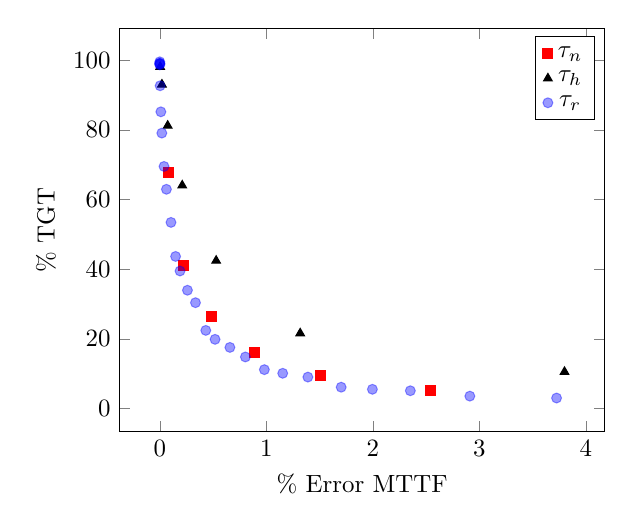
\begin{tikzpicture}[scale=0.9]
	    \begin{axis}[
	    	max space between ticks=30,
	        xlabel=\% Error MTTF,
	        ylabel=\% TGT
	      ]
	        \addplot[only marks,red,mark=square*] coordinates {
	            %(36.2283821103523, 1.131498272)
				%(10.8786955953901, 2.0599948)
				%(4.71755048985506, 2.926328112)
				(2.53732952715346, 5.310854768)
				(1.50720646565421, 9.43458592)
				(0.889037571328778, 16.21424912)
				(0.482749275852648, 26.56263144)
				(0.227135116763804, 41.153888896)
				(0.080131519802844, 67.78028296)
	        };
	        \addlegendentry{$\tau_n$}
	        \addplot[only marks,black,mark=triangle*] coordinates {
	            %(15.2851051823572, 5.065407888)
				(3.79933073326488, 10.55315872)
				(1.31806263244633, 21.607843456)
				(0.529240557949356, 42.444563712)
				(0.210743257691422, 64.033783088)
				(0.074347725814652, 81.17720832)
				(0.020278035133284, 92.977935568)
				(0.003661223540978, 98.040626224)
	        };
	        \addlegendentry{$\tau_h$}
	        \addplot[only marks,blue,opacity=0.4] coordinates {
				%(77.8389169546306, 00.861523664)
				%(53.6115397530694, 00.974922144)
				%(36.9436300763677, 01.152995024)
				%(19.6691222136954, 01.345055408)
				%(12.7403247404829, 01.904005072)
				%(10.3724266177443, 01.981527472)
				%(8.03701794393446, 02.251020576)
				%(5.44037121681866, 02.664600432)
				%(4.30725484221952, 02.719792576)
				(3.72475662384617, 03.040657568)
				(2.91070806039755, 03.582141952)
				(2.3520596495621, 05.126460944)
				(1.99594369221807, 05.54379928)
				(1.70283035361238, 06.145844688)
				(1.39021921620469, 09.046704608)
				(1.15419515287708, 10.136940352)
				(0.981883253585455, 11.18185456)
				(0.803778142429072, 14.81874224)
				(0.658367890409094, 17.559864032)
				(0.51894407728556, 19.877736832)
				(0.431973948594048, 22.436950304)
				(0.335262945633125, 30.392851952)
				(0.259775233206219, 33.959527536)
				(0.190106610385051, 39.480168544)
				(0.1484695504721, 43.655010816)
				(0.105215457995291, 53.421811456)
				(0.062484238182606, 62.918921632)
				(0.039821874791978, 69.478455152)
				(0.019324786397644, 79.03968496)
				(0.010279358713953, 85.14784744)
				(0.003281976729983, 92.620473392)
				(0.000287846441507, 98.61676752)
				(0.000074191212126, 98.965718112)
				(0.000009595371626, 99.49783808)
				(0.000001197524504, 99.10566392)
				(0.000000113524206, 98.86297784)
	        };
	        \addlegendentry{$\tau_r$}
	    \end{axis}
	\end{tikzpicture}
	\hspace{2em}
	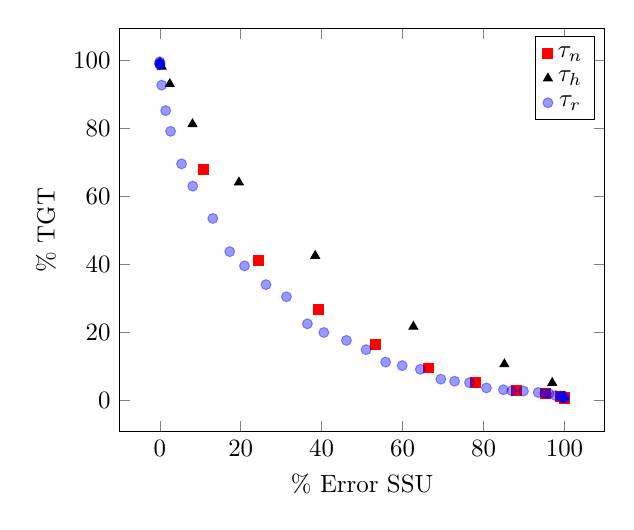
\begin{tikzpicture}[scale=0.9]
	    \begin{axis}[
	    	max space between ticks=30,
	        xlabel=\% Error SSU,
	        ylabel=\% TGT
	      ]
	        \addplot[only marks,red,mark=square*] coordinates {
		        (99.997820138894, 0.597874032)
				(99.9190691529866, 0.690664304)
				(98.9400899955787, 1.131498272)
				(95.4067719798257, 2.0599948)
				(88.2268633635062, 2.926328112)
				(78.0336186597343, 5.310854768)
				(66.3306911661053, 9.43458592)
				(53.4052347601024, 16.21424912)
				(39.2033637637174, 26.56263144)
				(24.49364613515, 41.153888896)
				(10.7288011862567, 67.78028296)
	        };
	        \addlegendentry{$\tau_n$}
	        \addplot[only marks,black,mark=triangle*] coordinates {
		        (99.870014762329, 1.004211856)
				(96.9670506258595, 5.065407888)
				(85.1329865668151, 10.55315872)
				(62.6536991241504, 21.607843456)
				(38.4026259662758, 42.444563712)
				(19.5569700042169, 64.033783088)
				(8.08755576023673, 81.17720832)
				(2.47742761181436, 92.977935568)
				(0.48941938798856, 98.040626224)
				(0.047212021885594, 99.235025232)
	        };
	        \addlegendentry{$\tau_h$}
	        \addplot[only marks,blue,opacity=0.4] coordinates {
				(99.9580166591334, 0.64276816)
				(99.9190691529866, 0.666556016)
				(99.5757277129978, 0.861523664)
				(99.3410468520113, 0.974922144)
				(98.9719987443901, 1.152995024)
				(97.7642769573984, 1.345055408)
				(96.1780559196505, 1.904005072)
				(95.1059074056779, 1.981527472)
				(93.4890534789559, 2.251020576)
				(89.8503866887823, 2.664600432)
				(86.9987828239507, 2.719792576)
				(84.9007507690672, 3.040657568)
				(80.7086068375894, 3.582141952)
				(76.5274064875573, 5.126460944)
				(72.8353681144488, 5.54379928)
				(69.4344925074714, 6.145844688)
				(64.3716966475546, 9.046704608)
				(59.8972972893015, 10.136940352)
				(55.8034316220035, 11.18185456)
				(50.9758925995969, 14.81874224)
				(46.1163102305292, 17.559864032)
				(40.5375554585927, 19.877736832)
				(36.475003450293, 22.436950304)
				(31.292572177161, 30.392851952)
				(26.2435957216562, 33.959527536)
				(20.9369931625395, 39.480168544)
				(17.2863722414051, 43.655010816)
				(13.1024452694755, 53.421811456)
				(8.13986333059419, 62.918921632)
				(5.38496052678585, 69.478455152)
				(2.67446059455362, 79.03968496)
				(1.45530814164037, 85.14784744)
				(0.468285490683692, 92.620473392)
				(0.041154518338355, 98.61676752)
				(0.010622504245067, 98.965718112)
				(0.001373917184128, 99.49783808)
				(0.000171469279963, 99.10566392)
				(0.000016255143934, 98.86297784)
	        };
	        \addlegendentry{$\tau_r$}
	    \end{axis}
	\end{tikzpicture}
	\captionof{figure}{Two graphs showing \%$TGT$ versus \%$MTTF$/$SSU$ when iterating each $\tau$}
	\label{fig:graph125}
\end{minipage}
% \end{figure}



\subsection{Choosing an appropriate $\tau_r$}
\label{sec:dijkstra}

The previous discussion shows that
a stopping criterion based on
a rate threshold appears to do
better than the other thresholds
we considered.
We now discuss a heuristic, based
on the building blocks of the model, to
try to select an appropriate value for
the rate threshold
$\tau_r$ so that only a relatively
small number of trees are generated
but the resulting error in the
dependability measures is small.
The method exploits the idea
that trees corresponding to the
most likely way the system fails
are the ones whose rates contribute most
to the computed dependability measures.
Exactly identifying these trees is
complicated,
so we instead use various
approximations and simplifying
assumptions to roughly determine
a value for $\tau_r$ that allows
such trees to be built but precludes
those with significantly smaller
rates.

Assume that the system consists
of highly reliable components
\cite{GSHNG:1992}
in the sense 
that the component
failure rates are much smaller than
the repair rates.
Suppose the system-operational
conditions require that
at least $\upsilon_i$ components
of each type $i$ are up
for the system to be operational,
and recall that $r_i$ is the
redundancy of type $i$.
Also suppose the system is currently
in a state with all components
up,
and we will focus only on trees
starting from such a state and that
lead to the system failing
in a single cascade.
The most likely way the
system fails in a single cascade is
when exactly $r_k - \upsilon_k + 1$ components
of some type $k$
fail (along with
other component types failing)
in the cascade.
We now want to roughly determine
what these trees look like
and their approximate rates.

% Recall that the rate $R(T)$ of a tree $T$
% with root type $i$ is
% determined by \eqref{eq:rate}.
% Define $R'(T) = \bar{\lambda}_i \rho$,
% where $\bar{\lambda}_i
% = \max_{e \in \mathcal{E}} \lambda_{i,e}$
% is the maximum failure rate for
% the root's type $i$
% over all the different environments,
% and $\rho$ is as defined in \eqref{eq:rate}.
Recall $R'(T)$ in \eqref{eq:R'}
is the product of the
maximum failure rate of the root and the
product of the component-affected
probabilities $\phi_{i,j}$ of
components that fail in
the cascade.
Now we want to
identify trees $T$ that lead to
the system failing in a single cascade
starting from an all-operational state
for which $R'(T)$ is large.
Since adding more nodes to
a tree will multiply its rate
by additional $\phi_{i,j}$ terms,
each of which is no greater than $1$,
such trees $T$
with large $R'(T)$
will
typically have not too many nodes
and the $\phi_{i,j}$ terms included
in $\rho$ from \eqref{eq:rate} will
often be relatively large.

We equivalently try to find
such trees $T$ with large $\ln(R'(T))$,
which converts the product $R'(T)$
into a sum of logs.
The advantage of this transformation
is that we can now use
a shortest-path algorithm on
an appropriately defined graph
to help identify
such trees.
Specifically,
construct a weighted graph
$G = (V,E,W)$,
where $V = \Omega$ is the set of
vertices, $E = \{ (i,j) : j \in \Gamma_i \}$
is its set of edges,
and $W = \{ w_{i,j} : (i,j) \in E \}$
is the set of weights (costs),
with $w_{i,j} = | \ln \phi_{i,j} |$.
Because $\ln \phi_{i,j} \leq 0$,
large $\phi_{i,j}$ corresponds to
small $w_{i,j}$.
To try to identify trees $T$ with large
$\ln(R'(T))$, we will build them
by first find//ing low-cost cycles
in $G$, which correspond roughly to
the most likely ways a component triggers
a cascade in which another component
of the same type fails.
Then repeat the cycles 
enough times so that the system
fails, thereby resulting in trees
for which $\ln(R'(T))$ should
be large.


For each type $i \in \Omega$ and
$j \in \Gamma_i$,
let $c_{j,i}$ be the cost of
the shortest path in the
weighted graph $G$ from vertex~$j$
to vertex $i$, and this can be determined
using Dijkstra's algorithm
(Section~24.3 of \cite{CLRS:2001}).
Let $c_i = \min_{j \in \Gamma_i}
(w_{i,j} + c_{j,i})$,
which is the cost of the
minimum-cost cycle from vertex $i$
back to itself.
Let $g_i = (g_{i,1}, g_{i,2},
\dots, g_{i,l_i})$ be the sequence of
nodes on this minimum cost cycle,
where $g_{i,1} = g_{i,l_i} = i$
and $l_i$ is the number
of vertices in the cycle
(including $i$ twice).
% This roughly corresponds to
% the product of the component-affected
% probabilities of
% a tree having a root of type $i$
% with exactly one more component of type $i$
% failing
% (along with some other component types).

Using the minimum-cost cycle $g_i$,
we then build a tree $T_i$ that is
a chain having
exactly $r_i - \upsilon_i + 1$
components of type $i$ failing
by repeating this minimum-cost cycle
$r_i - \upsilon_i$ times.
Specifically, let $g_i' =
(g_{i,2}, g_{i,3}, \ldots, g_{i,l_i})$,
which is the minimum-cost cycle $g_i$
with the starting vertex omitted.
Then $T_i$ is a chain with root
of type $i$, to which $g_i'$
is concatenated
$r_i - \upsilon_i$ times.
% Thus, $T_i$ has exactly
% $r_i - \upsilon_i + 1$ nodes
% of type $i$, along with nodes
% of other types.
We then use $T_i$ as
our approximation of
the tree corresponding to the
most likely way for the system
to fail from an all-operational state
with a single cascade triggered by a failure of
a component of type $i$.
For this tree $T_i$, we compute
$R'(T_i)$ as $\bar{\lambda}_i
a_i^{r_i - \upsilon_i}$,
where
$a_i = \prod_{j=1}^{l_i-1}
\phi_{g_{i,j}, g_{i,j+1}}$,
which is the product of
component-affected probabilities
along the minimum-cost
cycle.
Now we maximize over the types
to get
$\bar{R}' = \max_{i \in \Omega} R'(T_i)$,
and then set $\tau_r = \alpha \bar{R}'$,
where $\alpha$ is some constant.


\subsection{Extrapolation}

The method described in 
Section~\ref{sec:dijkstra}
tries to identify a ``good''
value for the rate threshold $\tau_r$,
but the resulting values for the MTTF
and the SSU may still have
significant errors.
We now consider a heuristic
to try to obtain better
estimates of the dependability
measures
using extrapolation.
The idea here is to compute
the MTTF and SSU for different
rate thresholds $\tau_r^{(1)} > 
\tau_r^{(2)} > \cdots >
\tau_r^{(b-1)}$
for some $b > 2$,
where $\tau_r^{(1)}$ is the
value of $\tau_r$ from
Section~\ref{sec:dijkstra}.
Let the corresponding values
for the MTTF and SSU be
$\mbox{MTTF}^{(j)}$
and $\mbox{SSU}^{(j)}$,
respectively,
for $j = 1, 2, \ldots, b-1$.
Then we extrapolate
$\mbox{MTTF}^{(j)}$
and $\mbox{SSU}^{(j)}$,
$j = 1, 2, \ldots, b-1$,
to obtain estimates
$\mbox{MTTF}^{(b)}$
and 
$\mbox{SSU}^{(b)}$.

In our experiments,
we set $b = ???$,
and set $\tau_r^{(j)} = 
\beta \tau_r^{(j-1)}$
for $j = 2, 3, \dots, b-1$,
where $0 < \beta < 1$ is a constant.
We performed the extrapolation
using \dots.





\section{Cloud-Computing Model}
\label{sec:cloud}



\section{Concluding Remarks}
\label{sec:conc}


\section{Possible Other Stuff?}
\subsection{MTTF Computation}
We remove the down-states from the matrix to speed up MTTF calculation.

\subsection{Bookmarks}
We do not store all failed components \varName{BFHist}, we simply multiply
until we hit a not-failed component. We cache BFH between succesive @  symbols
to get complement cumulative component affected probabilities in constant
time.


\section*{Acknowledgments}

This work has been supported
in part by
the National Science Foundation under
Grants No.\
CMMI-0926949 
and CMMI-1200065.
Any opinions, findings, and conclusions or recommendations
expressed in this material are those of the author and
do not necessarily reflect the views of the National
Science Foundation.


\bibliographystyle{plain}
\bibliography{mkn}

\end{document}